\begin{frame}[fragile]{Transaction serialization by RLP (Recursive Length Prefix)}
  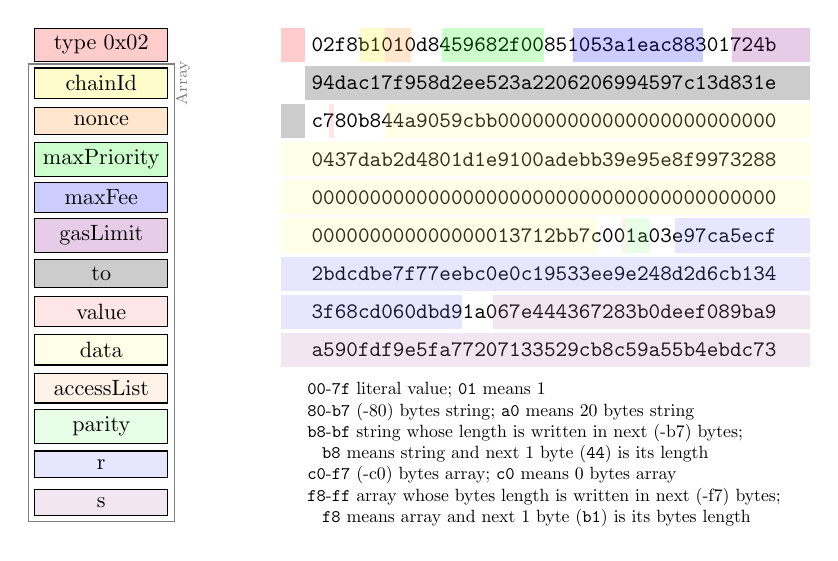
\begin{tikzpicture}[scale=0.8,every node/.style={transform shape}]
    \tikzstyle{field}=[minimum width=6em,minimum height=2.8ex,draw,fill opacity=0.2,text opacity=1.0]
    \node[field,fill=red] at (0,0) {type 0x02};
    \node[field,fill=yellow] at (0,-4ex) (chainId) {chainId};
    \node[field,fill=orange] at (0,-8ex) {nonce};
    \node[field,fill=green] at (0,-12ex) {maxPriority};
    \node[field,fill=blue] at (0,-16ex) {maxFee};
    \node[field,fill=violet] at (0,-20ex) {gasLimit};
    \node[field,fill=black] at (0,-24ex) {to};
    \node[field,fill=red!50] at (0,-28ex) {value};
    \node[field,fill=yellow!50] at (0,-32ex) {data};
    \node[field,fill=orange!50] at (0,-36ex) {accessList};
    \node[field,fill=green!50] at (0,-40ex) {parity};
    \node[field,fill=blue!50] at (0,-44ex) {r};
    \node[field,fill=violet!50] at (0,-48ex) {s};
      
    \draw[gray] (-3.3em,-2ex) rectangle (3.3em,-50ex);
    \node[rotate=90,gray] at (3.7em, -4ex) {{\scriptsize Array}};
    
\node at (20em,-0ex) {\texttt{02f8b1010d8459682f00851053a1eac88301724b}};
\node at (20em,-4ex) {\texttt{94dac17f958d2ee523a2206206994597c13d831e}};
\node at (20em,-8ex) {\texttt{c780b844a9059cbb000000000000000000000000}};
\node at (20em,-12ex) {\texttt{0437dab2d4801d1e9100adebb39e95e8f9973288}};
\node at (20em,-16ex) {\texttt{0000000000000000000000000000000000000000}};
\node at (20em,-20ex) {\texttt{000000000000000013712bb7c001a03e97ca5ecf}};
\node at (20em,-24ex) {\texttt{2bdcdbe7f77eebc0e0c19533ee9e248d2d6cb134}};
\node at (20em,-28ex) {\texttt{3f68cd060dbd91a067e444367283b0deef089ba9}};
\node at (20em,-32ex) {\texttt{a590fdf9e5fa77207133529cb8c59a55b4ebdc73}};
\node[align=left,scale=0.8] at (20em,-43ex) {
\texttt{00}-\texttt{7f} literal value; \texttt{01} means 1\\
\texttt{80}-\texttt{b7} ($\square$-80) bytes string; \texttt{a0} means 20 bytes string\\
\texttt{b8}-\texttt{bf} string whose length is written in next ($\square$-b7) bytes;\\ \hspace{0.5em} \texttt{b8} means string and next 1 byte (\texttt{44}) is its length\\
\texttt{c0}-\texttt{f7} ($\square$-c0) bytes array; \texttt{c0} means 0 bytes array\\
\texttt{f8}-\texttt{ff} array whose bytes length is written in next ($\square$-f7) bytes;\\ \hspace{0.5em} \texttt{f8} means array and next 1 byte (\texttt{b1}) is its bytes length
};
%\node at (20em,-36ex) {\texttt{80} = \texttt{80} + \texttt{0} bytes string, \ldots, \texttt{a0} = \texttt{80} + \texttt{20} bytes string};
%\node at (20em,-40ex) {\texttt{b8} = \texttt{b7} + \texttt{1} bytes string length (\texttt{44})};
%\node at (20em,-44ex) {\texttt{c0} = \texttt{c0} + \texttt{0} bytes array};
%\node at (20em,-48ex) {\texttt{f8} = \texttt{f7} + \texttt{1} bytes array length (\texttt{b1})};

\fill[red,opacity=0.2] (20em-11.9em,-0ex+1.8ex) rectangle (20em-11.9em +1.1em,-0ex-1.8ex); % type
\fill[yellow,opacity=0.2] (20em-11.9em +3.6em,-0ex+1.8ex) rectangle (20em-11.9em +3.6em+1.1em,-0ex-1.8ex); % chainId
\fill[orange,opacity=0.2] (20em-11.9em +4.7em,-0ex+1.8ex) rectangle (20em-11.9em +4.7em+1.2em,-0ex-1.8ex); % nonce
\fill[green,opacity=0.2] (20em-11.9em +7.3em,-0ex+1.8ex) rectangle (20em-11.9em +7.3em+4.6em,-0ex-1.8ex); % maxPriority
\fill[blue,opacity=0.2] (20em-11.9em +13.2em,-0ex+1.8ex) rectangle (20em-11.9em +13.2em+5.9em,-0ex-1.8ex); % maxFee
\fill[violet,opacity=0.2] (20em-11.9em +20.4em,-0ex+1.8ex) rectangle (20em-11.9em +20.4em+3.5em,-0ex-1.8ex); % gasLimit
\fill[black,opacity=0.2] (20em-11.9em +1.1em,-4ex+1.8ex) rectangle (20em-11.9em +1.1em+22.8em,-4ex-1.8ex); % to (first)
\fill[black,opacity=0.2] (20em-11.9em,-8ex+1.8ex) rectangle (20em-11.9em +1.1em,-8ex-1.8ex); % to (second)
\fill[red!50,opacity=0.2] (20em-11.9em +2.2em,-8ex+1.8ex) rectangle (20em-11.9em +2.2em+0.2em,-8ex-1.8ex); % value
\fill[yellow!50,opacity=0.2] (20em-11.9em +4.7em,-8ex+1.8ex) rectangle (20em-11.9em +23.9em,-8ex-1.8ex); % data (first)
\fill[yellow!50,opacity=0.2] (20em-11.9em,-12ex+1.8ex) rectangle (20em-11.9em +23.9em,-12ex-1.8ex); % data (second)
\fill[yellow!50,opacity=0.2] (20em-11.9em,-16ex+1.8ex) rectangle (20em-11.9em +23.9em,-16ex-1.8ex); % data (third)
\fill[yellow!50,opacity=0.2] (20em-11.9em,-20ex+1.8ex) rectangle (20em-11.9em +14.3em,-20ex-1.8ex); % data (fourth)
\fill[orange!50,opacity=0.2] (20em-11.9em +15.4em,-20ex+1.8ex) rectangle (20em-11.9em +15.4em+0.2em,-20ex-1.8ex); % accessList
\fill[green!50,opacity=0.2] (20em-11.9em +15.6em,-20ex+1.8ex) rectangle (20em-11.9em +15.6em+1.1em,-20ex-1.8ex); % parity
\fill[blue!50,opacity=0.2] (20em-11.9em +17.8em,-20ex+1.8ex) rectangle (20em-11.9em +23.9em,-20ex-1.8ex); % r (first)
\fill[blue!50,opacity=0.2] (20em-11.9em,-24ex+1.8ex) rectangle (20em-11.9em +23.9em,-24ex-1.8ex); % r (second)
\fill[blue!50,opacity=0.2] (20em-11.9em,-28ex+1.8ex) rectangle (20em-11.9em +8.2em,-28ex-1.8ex); % r (third)
\fill[violet!50,opacity=0.2] (20em-11.9em +9.6em,-28ex+1.8ex) rectangle (20em-11.9em +23.9em,-28ex-1.8ex); % s (first)
\fill[violet!50,opacity=0.2] (20em-11.9em,-32ex+1.8ex) rectangle (20em-11.9em +23.9em,-32ex-1.8ex); % s (second)
  \end{tikzpicture}
\end{frame}